\title{Assignment 2 \\ \small{Evolutionary Computing}}
\author{Chiel ten Brinke 3677133}
\documentclass[12pt]{article}
\usepackage{amssymb,amsmath,amsthm,enumerate,graphicx,float,lmodern,xparse}
\usepackage{hyperref}

\usepackage{tabularx,ragged2e,booktabs,caption}
\usepackage[T1]{fontenc}
\usepackage[utf8]{inputenc}
\usepackage{tabularx,ragged2e,booktabs,caption}
\newcolumntype{C}[1]{>{\Centering}m{#1}}
\renewcommand\tabularxcolumn[1]{C{#1}}
\usepackage{changepage}
%\usepackage[showframe=true]{geometry}

\newtheorem{theorem}{Theorem}[section]
\newtheorem{lemma}[theorem]{Lemma}
\newtheorem{proposition}[theorem]{Proposition}
\newtheorem{corollary}[theorem]{Corollary}

\theoremstyle{definition}
\newtheorem{definition}[theorem]{Definition}
\newtheorem{axiom}[theorem]{Axiom}
\newtheorem{example}[theorem]{Example}
\newtheorem{remark}[theorem]{Remark}

\NewDocumentCommand\set{mg}{%
    \ensuremath{\left\lbrace #1 \IfNoValueTF{#2}{}{\, \middle|\, #2} \right\rbrace}%
}

\newcommand{\co}{\texttt{counting ones}}
\newcommand{\lsco}{\texttt{linearly scaled counting ones}}
\newcommand{\tdt}{\texttt{tightly linked deceptive trap}}
\newcommand{\tnt}{\texttt{tightly linked non-deceptive trap}}
\newcommand{\rdt}{\texttt{randomly linked deceptive trap}}
\newcommand{\rnt}{\texttt{randomly linked non-deceptive trap}}

\setcounter{secnumdepth}{3}

\begin{document}
\maketitle

\section{Preliminary Notes}

\subsection*{Programming language}
The algorithms have been implemented in Cython~\cite{cython}.
Cython is a Python-like programming language which is translated into optimized
C/C++ code and compiled as Python extension modules.
This allows for very fast program execution, while keeping up the high programmer
productivity for which the Python language is well known.

We operate on 128 bit integers (GCC supports these), only using the first 100 bits.

\subsection*{Clustering Algorithm}
% Derive Jaccard distance from Mutual Information
We use a hierarchical clustering algorithm is that uses a mutual information based distance measure.
A set-theoretic interpretation of information (see Figure~\ref{fig:venn}) shows that
\[D(X,Y) = 1 - \frac{I(X;Y)}{H(X,Y)}.\]
In other words, we normalize $I(X;Y)$ and then we're able to substract it from 1 right away to get a distance measure instead of a similarity measure.
This is also known as the Jaccard distance.
For the distance between groups, we use the arithmetic average, as required.
\begin{figure}[!htb]
    \centering
    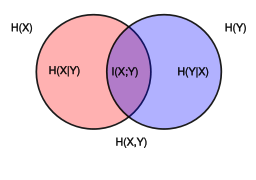
\includegraphics{images/venn.png}
    \caption{Individual $(H(X), H(Y))$, joint $(H(X, Y))$, and conditional entropies for a pair of correlated subsystems $X,Y$ with mutual information $I(X; Y)$.}
\label{fig:venn}
\end{figure}
% Refer to scipy
We outsource the clustering to the SciPy~\cite{scipy} library (scipy.cluster.hierarchy.linkage) using the Jaccard distance and arithmetical average.

\subsection*{Experimental Setup}
Since the implemention appears to be fast enough, the number of runs that is done to decide whether a population size is successful has been doubled.
So we consider problem to be solved reliably when 58 out of 60 independent runs find the optimal solution.

To get a better idea of how the population size influences the number of successes, we do not only show the population sizes that were used during the binary search, but with intervals of 20, we show the number of successes for each population size.

Nonetheless, the bisection search still has been implemented as required according to the instructions.
It has been used to determine the population size that is used to profile the fitness functions.

Other than the above, the assignment instructions have been followed precisely.
The obtained results can be found in the section below.


\section{Results}
\label{ssec:exp}
In Figure~\ref{fig:exp} the number of successes has been plot against the population size.
Table~\ref{tab:exp} shows information concerning the fitness function evaluations.

\begin{figure}[!htb]
    \centering
    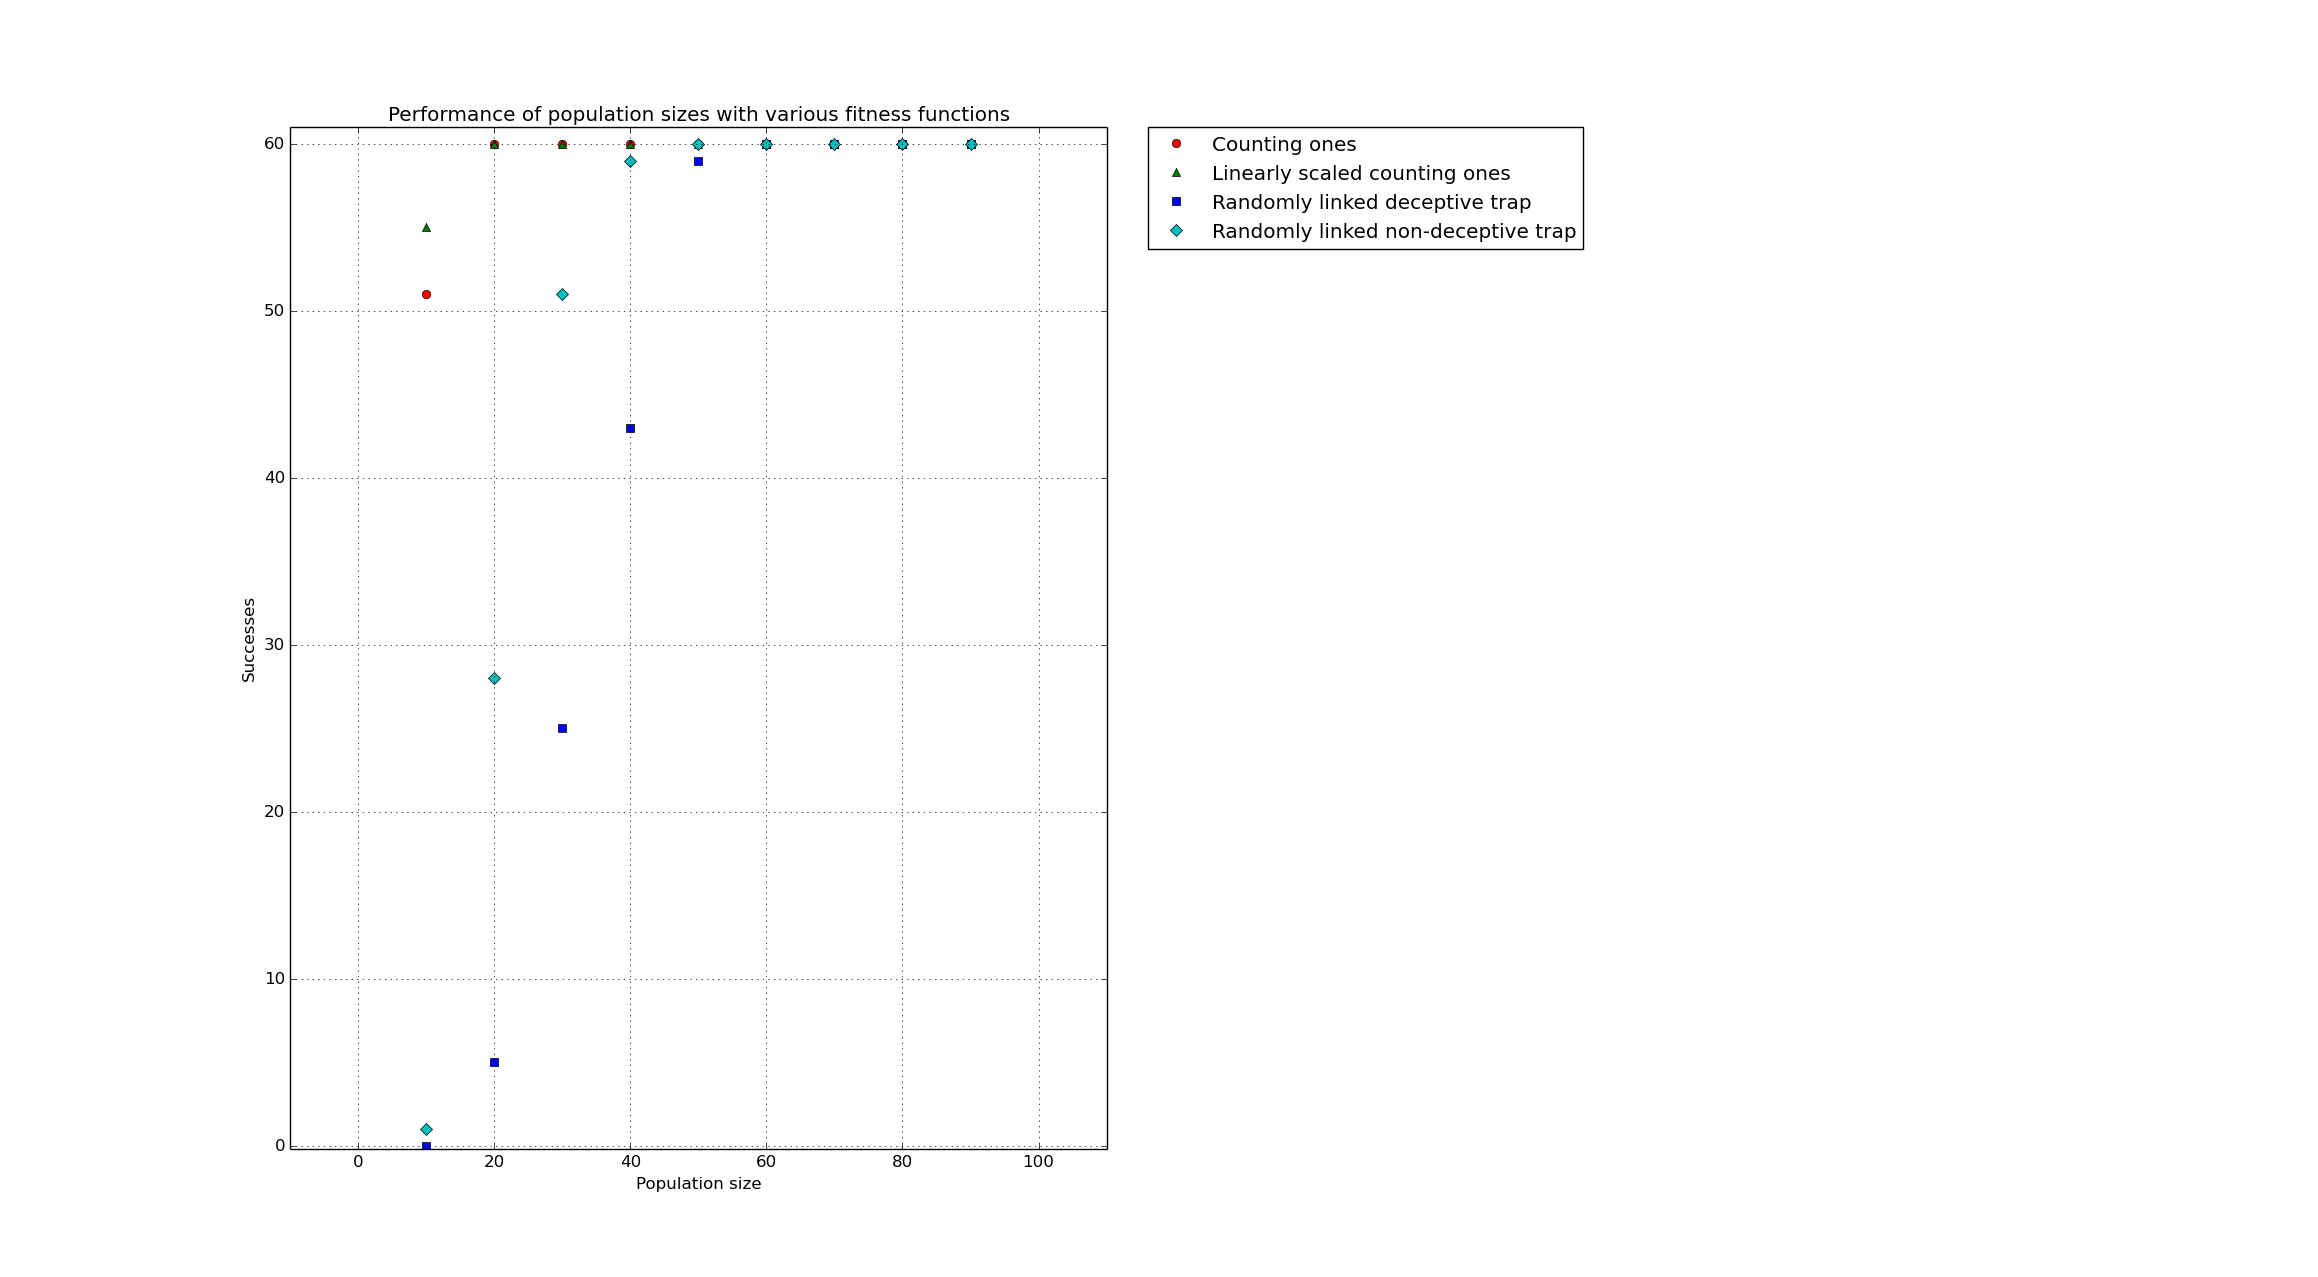
\includegraphics[totalheight=0.7\textheight]{images/exp.png}
    \caption{Number of success per population size}
\label{fig:exp}
\end{figure}

\begin{table}[!htb]
\begin{adjustwidth}{-2cm}{}
\centering
\begin{tabular}{lp{2.5cm}p{2.5cm}p{2.8cm}p{2.5cm}}
\toprule[1.5pt]
\bf Fitness function & \bf Population size & \bf Function evaluations & \bf Corresponding CPU time& \bf Generations\\\midrule
Counting ones & 10 & 20010 & 0.006 seconds & 5 \\
Linearly scaled Counting ones & 20 & 40020 & 0.008 seconds & 5 \\
Randomly linked deceptive trap & 50 & 200050 & 0.354 seconds & 10 \\
Randomly linked non-deceptive trap & 50 & 160050 & 0.272 seconds & 8 \\
\bottomrule[1.25pt]
\end{tabular}\par
\bigskip
\captionof{table}{Fitness function evaluations}
\label{tab:exp}
\end{adjustwidth}
\end{table}

% Constructs: to be expected, intuitively clear, not surprising, evident
\paragraph{Observations}
The first observation one can make is that this algorithm outperforms all algorithms of the
previous practical assignment by far.
Even the randomly linked trap functions are solved easily.
Neither the number of generations or the population size has to be large in order to
converge to the global optimum.

Unsurprisingly, the non-deceptive trap function is easier to solve than the deceptive version,
and both trap functions are harder than the counting ones variations.

We also observe there is more overhead in computional time.
The CPU time required is somewhat comparable to the results of the previous practical assignment,
while the number of function evaluations is lower.
This may be caused by transformations between our data structures and those of the SciPy library.
If the clustering algorithm would have been optimized for our datastructures,
it is likely that the computional time would be even lower.

\paragraph{Conclusion}
Experimental results for randomly linked trap functions show that the LTGA can solve hard functions efficiently without having apriori knowledge about the position of the linked variables on the solutions.
The LTGA algorithm appears to take a good compromise between complexity of the linkage model and search efficiency, compared to the setups that were tested in the first practical assignment.
This supports the conclusion of Dirk Thierens in \emph{The Linkage Tree Genetic Algorithm}~\cite{dirk}.


\begin{thebibliography}{9}

\bibitem{cython}
R. Bradshaw, S. Behnel, D. S. Seljebotn, G. Ewing, et al.,
The Cython compiler, \url{http://cython.org}.

\bibitem{scipy}
Eric Jones and Travis Oliphant and Pearu Peterson and others,
SciPy: Open source scientific tools for Python, \url{http://www.scipy.org}.

\bibitem{dirk}
Dirk Thierens,
The Linkage Tree Genetic Algorithm.
Institute of Information and Computing Sciences
Universiteit Utrecht, The Netherlands,
2010.

\end{thebibliography}


\end{document}
